\documentclass[a4paper]{article} 
\addtolength{\hoffset}{-2.25cm}
\addtolength{\textwidth}{4.5cm}
\addtolength{\voffset}{-3.25cm}
\addtolength{\textheight}{5cm}
\setlength{\parskip}{0pt}
\setlength{\parindent}{0in}

\usepackage{blindtext} % Package to generate dummy text
\usepackage{charter} % Use the Charter font
\usepackage[utf8]{inputenc} % Use UTF-8 encoding
\usepackage{microtype} % Slightly tweak font spacing for aesthetics
\usepackage[english]{babel} % Language hyphenation and typographical rules
\usepackage{amsthm, amsmath, amssymb} % Mathematical typesetting
\usepackage{float} % Improved interface for floating objects
\usepackage{subcaption}
\usepackage[final, colorlinks = true, 
linkcolor = black, 
citecolor = black]{hyperref} % For hyperlinks in the PDF
\usepackage{graphicx, multicol} % Enhanced support for graphics
\usepackage{xcolor} % Driver-independent color extensions
\usepackage{marvosym, wasysym} % More symbols
\usepackage{rotating} % Rotation tools
\usepackage{censor} % Facilities for controlling restricted text
\newcommand{\note}[1]{\marginpar{\scriptsize \textcolor{red}{#1}}} % Enables comments in red on margin
\definecolor{colkeyword}{rgb}{0,0.4,0}
\definecolor{colname}{rgb}{0.4,0.4,0}
\definecolor{coltype}{rgb}{0.4,0,0.4}
\definecolor{coloperators}{rgb}{0,0,1.0}
\definecolor{colscopes}{rgb}{0.4,0,0}

% Title Page
\title{Documentation Lean Hammer}
\author{Phillip Lippe}


\begin{document}
\maketitle
\tableofcontents
\newpage

\section{Specific pipeline DTT to FOL}
\subsection{Approach}
The first version of the Lean hammer implements a direct translation from DTT to FOL. The approach follows the \href{https://link.springer.com/article/10.1007/s10817-018-9458-4}{Coq hammer paper} by introducing an intermediate representation
\subsection{Implementation}
\subsubsection{Code structure}
The code is split into multiple files
\begin{itemize}
	\item \texttt{leanhammer.lean}: Main file combining all functions for testing. In here, we include examples of translation, and show the usage of the overall system.
	\item \texttt{problem\_translation.lean}: Summarizes the steps for translating a problem into FOF. Note that this file should mostly be independent of the actual encoding of the first-order logic.
	\item \texttt{premise\_selection.lean}: Implementation of strategies for selecting the most relevant premises/axioms. Still in a very early form. Might be moved into C/C++ code for performance gain. 
	\item \texttt{import\_export.lean}: Handling functions for the import and export of files (communication to first-order provers)
\end{itemize}

Next to the general files, there are several functions that directly interact with the underlying FOF encoding. Currently, only the TPTP3 encoding is fully supported that can be processed by theorem provers like E. The implementation for that is structured as follows:
\begin{itemize}
	\item \texttt{tptp.lean}: Summarizes data structures for simple first-order formula and their representation in the TPTP format
	\item \texttt{translation\_tptp.lean}: Functions for translating expressions into FOF. This include the hammer functions \textit{F}, \textit{C} and \textit{G}. 
	\item \texttt{simplification\_tptp.lean}: Simplification functions for TPTP encoded first-order formula 
\end{itemize}

\subsubsection{Encoding of inductive declarations}
\subsection{Examples}
The file \texttt{leanhammer.lean} contains a few examples of translating DTT to FOL. For explanation purpose, Figure~\ref{fig:fol_example_declaration} shows a sample translation example where we want to prove that the second Fibonacci number is equals to 2.
\begin{figure}[ht!]
	\centering
	\begin{subfigure}{0.33\textwidth}
		\centering
		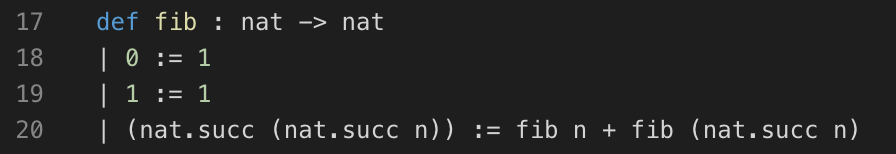
\includegraphics[width=\textwidth]{figures/fol_example_fib_definition.png}
		\caption{Sample inductive declaration}
		\label{fig:fol_example_declaration}
	\end{subfigure}
	\hspace{1mm}
	\begin{subfigure}{0.65\textwidth}
		\centering
		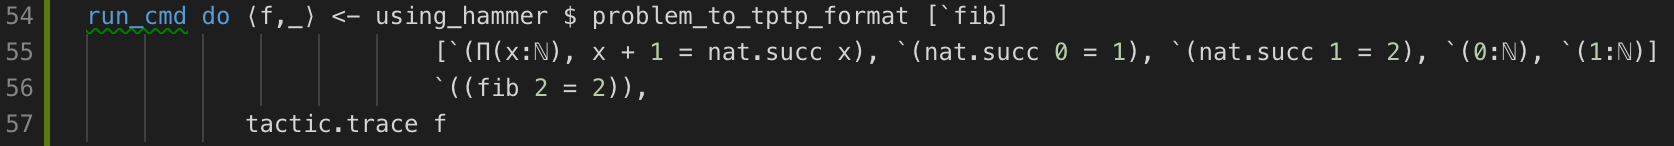
\includegraphics[width=\textwidth]{figures/fol_example_call.png}
		\caption{Sample translation problem}
		\label{fig:fol_example_translation}
	\end{subfigure}
	\caption{FOL translation example in Lean. The code can be found in the file \texttt{leanhammer.lean}. The left side shows the inductive declaration of \texttt{fib}, and the right the call for translating this into plain FOL in TPTP encoding. }
	\label{fig:fol_example}
\end{figure}

The main function that is used is \texttt{problem\_to\_tptp\_format}. This function takes as first argument a list of declarations that are eventually relevant for the conjecture and should be included in the translation. In our case, we want to translate the inductive declaration of the Fibonacci numbers as shown in Figure~\ref{fig:fol_example_declaration}. The second argument is a list of expressions that should be translated as clauses. Here, we for example have to define that 0 and 1 are natural numbers. If we would leave these out, we will not be able to find a proof as the clause implementing \texttt{fib} in FOL has as pre-condition that the argument is of type \texttt{nat}. The last expression we enter to the translation process is of course the conjecture. By tracing the output of the function, we see the translated construct in text form, which can be used for other theorem provers. \\

To use this translation, copy output to the file \texttt{test\_problem.tptp} (note that the name of the file can be changed).
Run a theorem prover like E on this file by executing the command \texttt{./eprover --auto --tptp3-in \textit{file/to/}test\_problem.tptp}. If everything worked out correctly, E finds a proof in a few milliseconds.
\subsection{Open issues}
\begin{itemize}
	\item Up till now, the user has to specify by himself which declarations and expressions should be translated besides the conjecture. This process should be automated by a retrieving all possible clauses/declarations that are somehow connected with the conjecture, and then filtering/ranking these to only take the $N$ most relevant ones. Code based on an old version of Lean can be found \href{https://github.com/robertylewis/relevance_filter/tree/dev_lean_reparam}{here}, and the file \texttt{premise\_selection.lean} might be a good starting point.
	\item The translation of inductive declarations works fine in the Lean hammer. However, plain declarations like:\\
	\texttt{def sum\_two (x:$\mathbb{N}$) (y:$\mathbb{N}$) :$\mathbb{N}$ := x+y}\\
	cause troubles in the translation problem. Lean represents these functions as lambda expressions although we need it in pi notation (for all \texttt{x} and \texttt{y}, \texttt{sum\_two x y = x + y}). This translation needs to be integrated into the hammer. For debugging, a quick fix is to write all declarations inductively.
	\item Currently, the interaction to the theorem prover is in a debug stage where the user needs to copy the output of Lean into a file, and run E on it. In future, this process should be automated by an IO import/export to theorem provers.
	\item In relation to the previous points, once the IO communication with the theorem provers is automated, a proof reconstruction needs to be implemented. This would help the user to understand the proof, and provide him a way of implementing this proof in Lean.
	\item Another missing point is the translation of inductive types like \texttt{list}. Currently, these types are not supported.
\end{itemize}
\section{General pipeline}
To support theorem provers of different input levels (TF0, TF1, TH0, TH1), the generalized version of the Lean hammer is planed to follow a pipeline which successively translates the Dependent Type Theory to FOL. The pipeline is visualized in Figure~\ref{fig:pipeline}.
\begin{figure}[ht!]
	\centering
	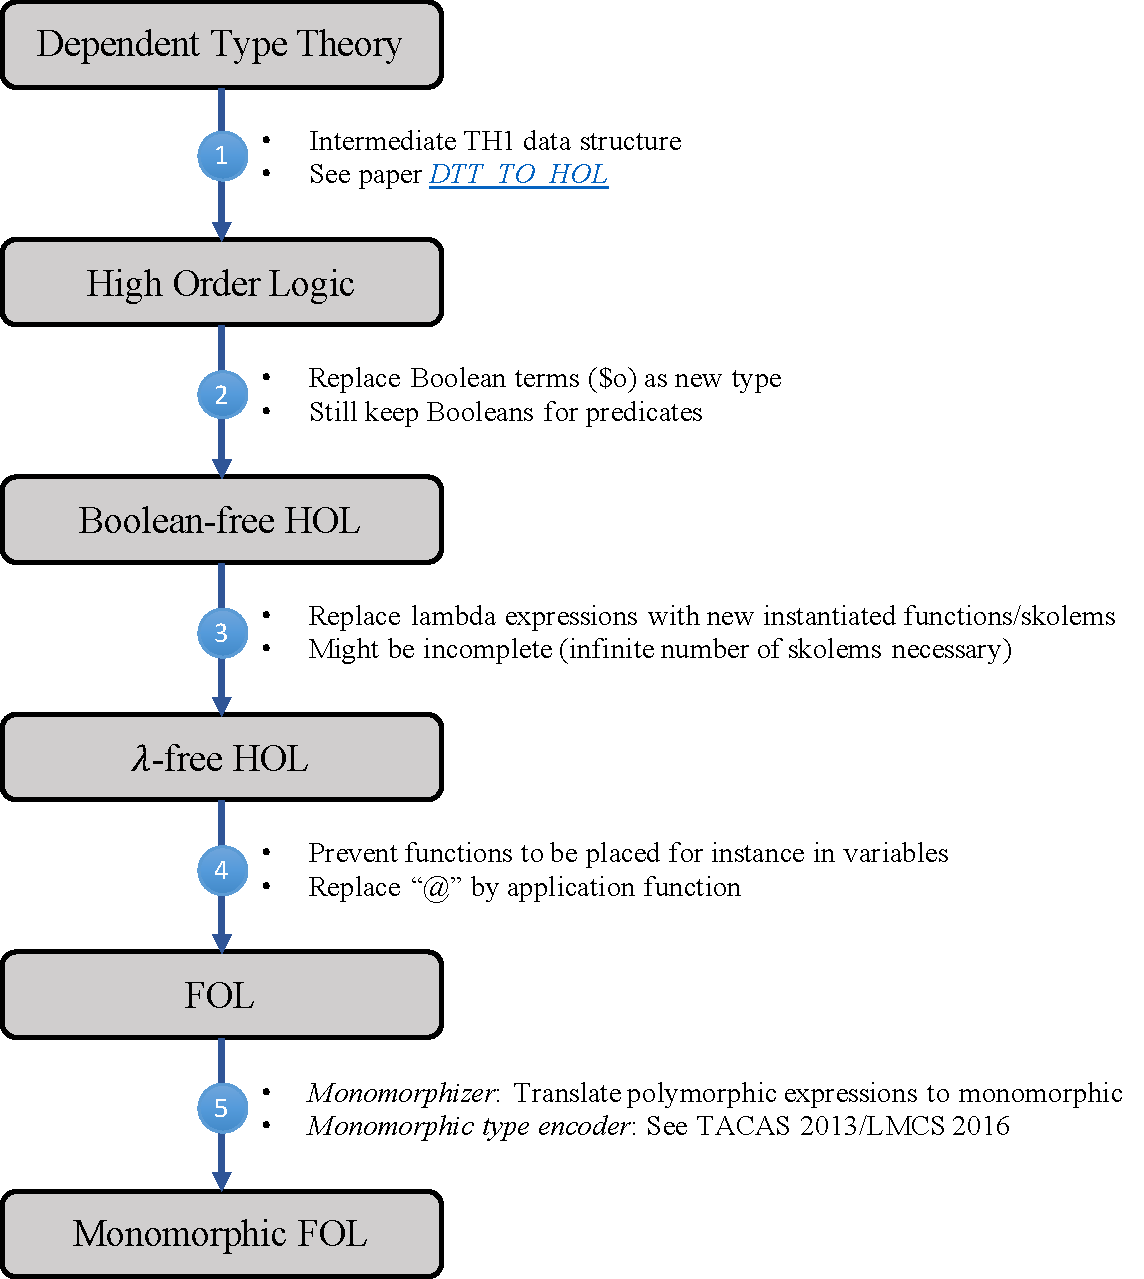
\includegraphics[width=0.45\textwidth]{figures/pipeline_DTT_HOL.pdf}
	\caption{General overview of the translation pipeline from Dependent Type Theory to different logic forms.}
	\label{fig:pipeline}
\end{figure}
\subsection{Dependent Type Theory to High Order Logic}
Paper DTT to HOL: \href{https://link.springer.com/chapter/10.1007/BFb0037108}{paper}. We introduce an intermediate data structure based on TH1 which can be parsed. 
\subsection{High Order Logic to Boolean-free HOL}
\subsection{Boolean-free HOL to $\lambda$-free HOL}
\subsection{$\lambda$-free HOL to FOL}
\subsection{FOL to monomorphic FOL}

\appendix
\section{FOL examples}
\begin{verbatim}
fof('_fresh.265.4460',
axiom,
(t(a(a('has_one.one',
'nat'),
'nat.has_one'),
'nat'))).

fof('_fresh.265.4459',
axiom,
(t(a(a('has_zero.zero',
'nat'),
'nat.has_zero'),
'nat'))).

fof('_fresh.265.4455',
axiom,
((a(a(a('bit0',
'nat'),
'nat.has_add'),
a(a('has_one.one',
'nat'),
'nat.has_one'))
= a('nat.succ',
a(a('has_one.one',
'nat'),
'nat.has_one'))))).

fof('_fresh.265.4454',
axiom,
(t(a('nat.succ',
a(a('has_one.one',
'nat'),
'nat.has_one')),
'nat'))).

fof('_fresh.265.4453',
axiom,
((a(a('has_one.one',
'nat'),
'nat.has_one')
= a('nat.succ',
a(a('has_zero.zero',
'nat'),
'nat.has_zero'))))).

fof('_fresh.265.4452',
axiom,
(t(a('nat.succ',
a(a('has_zero.zero',
'nat'),
'nat.has_zero')),
'nat'))).

fof('_fresh.265.4450',
axiom,
(! [V1 /* _fresh.265.4451 */] :
((t(V1,
'nat'))
=> (t(a('fib',
V1),
'nat'))))).

fof('_fresh.265.4447',
axiom,
((a('fib',
a(a('has_zero.zero',
'nat'),
'nat.has_zero'))
= a(a('has_one.one',
'nat'),
'nat.has_one')))).

fof('_fresh.265.4444',
axiom,
((a('fib',
a(a('has_one.one',
'nat'),
'nat.has_one'))
= a(a('has_one.one',
'nat'),
'nat.has_one')))).

fof('_fresh.265.4437',
axiom,
(! [V1 /* _fresh.265.4438 */] :
((t(V1,
'nat'))
=> ((a('fib',
a('nat.succ',
a('nat.succ',
V1)))
= a(a(a(a('has_add.add',
'nat'),
'nat.has_add'),
a('fib',
V1)),
a('fib',
a('nat.succ',
V1)))))))).

fof('problem_conjecture',
conjecture,
((a('fib',
a(a(a('bit0',
'nat'),
'nat.has_add'),
a(a('has_one.one',
'nat'),
'nat.has_one')))
= a(a(a('bit0',
'nat'),
'nat.has_add'),
a(a('has_one.one',
'nat'),
'nat.has_one'))))).
\end{verbatim}
\end{document}